%%
%% This is file `sample-sigplan.tex',
%% generated with the docstrip utility.
%%
%% The original source files were:
%%
%% samples.dtx  (with options: `sigplan')
%% 
%% IMPORTANT NOTICE:
%% 
%% For the copyright see the source file.
%% 
%% Any modified versions of this file must be renamed
%% with new filenames distinct from sample-sigplan.tex.
%% 
%% For distribution of the original source see the terms
%% for copying and modification in the file samples.dtx.
%% 
%% This generated file may be distributed as long as the
%% original source files, as listed above, are part of the
%% same distribution. (The sources need not necessarily be
%% in the same archive or directory.)
%%
%% Commands for TeXCount
%TC:macro \cite [option:text,text]
%TC:macro \citep [option:text,text]
%TC:macro \citet [option:text,text]
%TC:envir table 0 1
%TC:envir table* 0 1
%TC:envir tabular [ignore] word
%TC:envir displaymath 0 word
%TC:envir math 0 word
%TC:envir comment 0 0
%%
%%
%% The first command in your LaTeX source must be the \documentclass command.
\documentclass[sigplan,screen]{acmart}
%% NOTE that a single column version is required for 
%% submission and peer review. This can be done by changing
%% the \doucmentclass[...]{acmart} in this template to 
% \documentclass[manuscript,screen,review]{acmart}
%% 
%% To ensure 100% compatibility, please check the white list of
%% approved LaTeX packages to be used with the Master Article Template at
%% https://www.acm.org/publications/taps/whitelist-of-latex-packages 
%% before creating your document. The white list page provides 
%% information on how to submit additional LaTeX packages for 
%% review and adoption.
%% Fonts used in the template cannot be substituted; margin 
%% adjustments are not allowed.
%%
%% \BibTeX command to typeset BibTeX logo in the docs
\AtBeginDocument{%
  \providecommand\BibTeX{{%
    \normalfont B\kern-0.5em{\scshape i\kern-0.25em b}\kern-0.8em\TeX}}}

%% Rights management information.  This information is sent to you
%% when you complete the rights form.  These commands have SAMPLE
%% values in them; it is your responsibility as an author to replace
%% the commands and values with those provided to you when you
%% complete the rights form.
%\setcopyright{acmcopyright}
%\copyrightyear{2018}
%\acmYear{2018}
%\acmDOI{XXXXXXX.XXXXXXX}

%% These commands are for a PROCEEDINGS abstract or paper.
%\acmConference[Conference acronym 'XX]{Make sure to enter the correct
 % conference title from your rights confirmation emai}{June 03--05,
 % 2018}{Woodstock, NY}
%
%  Uncomment \acmBooktitle if th title of the proceedings is different
%  from ``Proceedings of ...''!
%
%\acmBooktitle{Woodstock '18: ACM Symposium on Neural Gaze Detection,
%  June 03--05, 2018, Woodstock, NY} 
%\acmPrice{15.00}
%\acmISBN{978-1-4503-XXXX-X/18/06}

%%
%% For managing citations, it is recommended to use bibliography
%% files in BibTeX format.
%%
%% You can then either use BibTeX with the ACM-Reference-Format style,
%% or BibLaTeX with the acmnumeric or acmauthoryear sytles, that include
%% support for advanced citation of software artefact from the
%% biblatex-software package, also separately available on CTAN.
%%
%% Look at the sample-*-biblatex.tex files for templates showcasing
%% the biblatex styles.
%%

%%
%% The majority of ACM publications use numbered citations and
%% references.  The command \citestyle{authoryear} switches to the
%% "author year" style.
%%
%% If you are preparing content for an event
%% sponsored by ACM SIGGRAPH, you must use the "author year" style of
%% citations and references.
%% Uncommenting
%% the next command will enable that style.
%%\citestyle{acmauthoryear}

%%
%% end of the preamble, start of the body of the document source.
\begin{document}

%%
%% The "title" command has an optional parameter,
%% allowing the author to define a "short title" to be used in page headers.
\title{A Survey of Multi-hop Reading Comprehension approaches using Graph Neural Networks}

%%
%% The "author" command and its associated commands are used to define
%% the authors and their affiliations.
%% Of note is the shared affiliation of the first two authors, and the
%% "authornote" and "authornotemark" commands
%% used to denote shared contribution to the research.
\author{Ajay Narayanan}

\author{Constantin Weberpals}

\author{Tim Bruckdorfer}


%%
%% By default, the full list of authors will be used in the page
%% headers. Often, this list is too long, and will overlap
%% other information printed in the page headers. This command allows
%% the author to define a more concise list
%% of authors' names for this purpose.
% \renewcommand{\shortauthors}{Ajay Narayanan, Constantin Weberpals, Tim Bruckdorfer}

%%
%% The abstract is a short summary of the work to be presented in the
%% article.
\begin{abstract}
  Fill in your abstract here. Summarize your paper and highlight the most important findings.
\end{abstract}

\maketitle

\section{Introduction}
%TODO
% Start writing your paper here and don't forget to include citations. Example: GCN \cite{RN2}
The task of Machine Reading Comprehension, or MRC is an active area of research in the field of Natural Language Processing. 
The basic goal of MRC is to develop systems that can read and comprehend unstructured passages and answer questions based on them. 

Recently, there has been a lot of interest in the task of multi-hop reading comprehension (MHRC), 
where the answer to a question is not directly stated in a single passage, but can be inferred by combining information from multiple documents.
To this end, a number of datasets have been proposed, such as HotpotQA \cite{RN116}, QAngaroo \cite{RN115}, and MuSiQue \cite{RN167}. Some datasets 
also include supporting facts, whose extraction could be seen as providing explainability for MHRC tasks  \cite{RN116} \cite{RN106}.

To solve the task of MHRC, a number of approaches have been proposed, which can be broadly classified into two categories:
Graph-based approaches \cite{RN81} \cite{RN117} \cite{RN118} \cite{RN122} \cite{RN119} \cite{RN91} and Non-graph-based approaches. Most of the methods
can be basically decomposed into a Retrieval phase and a Reading phase \cite{RN166}. Graph-based approaches can be effective for this task because they 
enable the modeling of complex relationships between entities \cite{RN23}, and provide the integration of global evidence. They can also mimic human 
reasoning processes \cite{RN35}.

\begin{figure}[h] % 'h' for "here", can be replaced with other placement specifiers
  \centering
  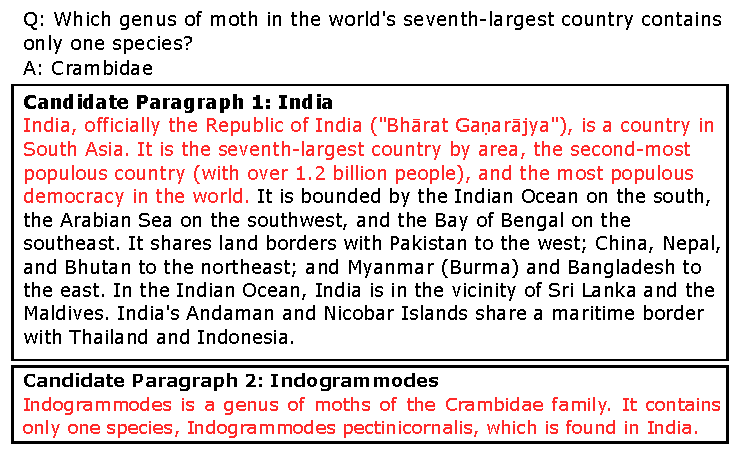
\includegraphics[width=\linewidth]{fig/fig_1_hotpot_example.pdf} % Adjust 'width' as needed
  \caption{A Sample question from the HotpotQA dataset}
  \label{fig:yourlabel} % For referencing the figure in the text
\end{figure}

%TODO: figure of example multi-hop reasoning problem from HotpotQA

%TODO: brief description of non-graph-based approaches

The first step in Graph-based approaches is to construct either an entity graph \cite{RN81} \cite{RN117} \cite{RN122} \cite{RN141} \cite{RN91} \cite{RN130} 
or a hierarchical graph \cite{RN124} \cite{RN119} \cite{RN130}, to model the relationships in the texts. Once this is done, a GNN-based 
reasoning module is used to perform multi-hop reasoning over the graph, and finally a prediction module is used to predict answers \cite{RN23}.
%TODO: expand this paragraph

Recently, there have been arguments as to whether GNNs are actually necessary for MHRC. Shao et al. (2020) \cite{RN127} argue that 
a graph structure may not be necessary with proper use of pre-trained models, and that the graph structure can be regarded as task-specific 
prior knowledge. Groenveld et al. (2020) \cite{RN126} showed that a simple BERT-based model can outperform a Graph-based model on the HotpotQA dataset,
and that supporting sentence identification in HotpotQA might not be a multi-hop problem at all. Wu et al. (2021) \cite{RN106} suggested that
the paragraph retrieval stage might be more important than the reasoning stage in MHRC, and that the reasoning stage might not be a multi-hop problem.
%TODO: motivation for survey - is GNN necessary for MHRC?
%TODO: mention Min et al. argument about the MHRC Dataset problem

In this paper, we present a survey of various approaches that have been proposed for MHRC, with a focus on Graph-based approaches. We also try to
address the question of whether GNNs are actually necessary for MHRC. We first present a taxonomy of the various approaches, and then discuss the
core concepts of MHRC. We then present a detailed discussion of the various approaches, and finally conclude with a discussion of the open problems 
and future directions.
%TODO: contributions of survey

\section{Background}
In this section we intruduce the core concepts of multi-hop reasoning and graph neural networks that prior research has established.  

%TODO
\subsection{Machine Reading Comprehension and Multi-hop QA}
The goal of MRC is to enable machines to answer questions based on a given text or set of texts, requiring a deep understanding of both the content and context of the input material, which 
requires advanced NLP techniques, such as semantic analysis, context understanding, and language modeling \cite{RN208}. MRC represents a significant challenge in AI and NLP, as it requires systems to not only process language but also to comprehend and infer meaning in a way comparable to human understanding.

Multi-hop question answering (QA) is a challanging aspect of MRC that requires multi-step reasoning over multiple passages to find the answer and supporting evidence \cite{RN165}.
It is a crucial component of natural language processing (NLP) and AI systems, with a wide range of applications, as it requires models to connect multiple pieces of 
evidence to answer complex questions. Therefore, it can be used for tasks such as document and timeline summarization \cite{RN202} \cite{RN201}.
To improve the performance of multi-hop QA models, different model architectures such as hybrid models or TransferNet, which supports both label and text relations in a unified framework \cite{RN164} \cite{RN133}. 
The development of better models was further encouraged through the availability of high quality data sets \cite{RN116} \cite{RN115}
Studies collectively highlight the importance of multi-hop QA in enhancing the reasoning and inference skills of NLP models across various domains. 
A notable development in multi-hop QA is the application of Graph Neural Networks. The multi-hop attention mechanism in GNNs, for instance, has improved information aggregation, making these 
models more effective and accurate in complex reasoning tasks \cite{RN109}. These advancements have significantly improved the performance of multi-hop QA models, making them more effective and accurate.

\subsection{Multi-hop QA Datasets}
The advancement of multi-hop QA has been greatly facilitated by the introduction of specific datasets designed to test and refine the reasoning capabilities of AI models. 
Notable among these are HotpotQA, WikiHop, and ComplexWebQuestions, each presenting unique challenges and features \cite{RN115}\cite{RN116}\cite{RN104}.
These datasets have been instrumental in benchmarking the performance and progress in the field. 



\begin{table*}[ht]
  \centering
  \begin{tabular}{|l|l|p{3cm}|p{3cm}|l|}
  \hline
  \textbf{Dataset}            & \textbf{Introduced by} & \textbf{Description} & \textbf{Key Features} & \textbf{Reasoning Types} \\ \hline
  HotpotQA           & Yang et al., 2018 & A large-scale dataset requiring understanding and synthesis of information from multiple paragraphs. & Provides questions, answers, and supporting facts for explainable QA. & Comparison, bridge, intersection \\ \hline
  WikiHop            & Welbl et al., 2018 & Constructed from Wikipedia articles, focusing on indirect inference across multiple documents. & Tests the ability to navigate and reason across linked documents. & Long-range dependencies \\ \hline
  ComplexWebQuestions & Talmor \& Berant, 2018 & Requires performing intricate queries over a large web-scale knowledge base. & Synthesizes information from various web sources. & Web-based, domain-specific knowledge \\ \hline
  \end{tabular}
  \caption{Overview of Multi-hop QA Datasets}
  \label{table:multihop_datasets}
  \end{table*}
  
  
  

\subsection{Graph Neural Networks}

A range of studies have contributed to the advancement of Graph Neural Networks (GNNs). These networks have emerged 
as a powerful tool for machine learning on graph-structured data, extending the capabilities of traditional neural networks to complex relationships and 
interdependencies encoded in graphs. The work of Gori et al. \cite{RN203} and Scarselli et al. \cite{RN204}, who proposed a framework for applying neural networks directly to graphs 
layed the foundation for further developments in that field.

GNNs are designed to capture the relational information inherent in the graphical representation of data \cite{RN205}. This makes them particularly 
well-suited for applications where data points are interrelated, such as social networks, molecular structures, and communication networks \cite{RN206}.

A core principle of GNNs lies in their ability to learn representations for nodes by incorporating neighborhood information. Through mechanisms such as neighborhood aggregation or message passing, nodes update their 
representations by adapting features from adjacent nodes \cite{RN207}. This iterative process facilitates information flow across the network, enabling the GNN to capture complex 
relational patterns \cite{RN15}. One of the most prominent variants of GNNs is the Graph Convolutional Network (GCN), introduced by Kipf and Welling (2016). 
GCNs generalize the concept of convolution from grid-like data (e.g., images) to graphs, enabling efficient feature extraction from graph data \cite{RN209}. Another notable variant is the 
Graph Attention Network (GAT), introduced by Veličković et al. (2018). GATs incorporate attention mechanisms in the aggregation process, allowing for more nuanced weighting of neighbor contributions, which 
enhances the model's ability to focus on important features in the graph \cite{RN7}.

GNNs have not only enriched the landscape of neural network architectures but have also opened new avenues in various domains that deal with complex relational data. Their continued evolution and integration with other AI fields makes them an interesting topic to investigate in the context of multi-hop reasoning.

\section{Taxonomy}
%TODO

\section{Core Concepts}
%TODO
\subsection{An Overview of Graph based approaches}
For the purposes of understanding Graph based approaches, we will consider the following models:
DFGN \cite{RN122}, HGN \cite{RN119}, CogQA \cite{RN118} and DRN \cite{RN142}. We will also compare them with 
a couple of leading non-graph-based approaches: Beam Retriever (Current SOTA for HotpotQA Distractor Setting) \cite{RN105} and
HopRetriever \cite{RN149}.


\subsection{An evaluation of Graph based approaches}

\subsection{Analysis of Multi-hop Datasets}
%TODO graph based models are still pretty good in the fullwiki setting - maybe that is a potential future direction?

\section{Related Work}
%TODO

\section{Conclusion}
%TODO

% add bibliography
\bibliographystyle{ACM-Reference-Format}
\bibliography{bib.bib}

\end{document}
\endinput
%%
%% End of file
